\documentclass{beamer}
\setbeamertemplate{navigation symbols}{}
\usetheme{Frankfurt}

\usepackage{listings}
\lstdefinestyle{code}{
  language       = C++,
  basicstyle      = \footnotesize\ttfamily\color{gray},
  numbers         = left,
  tabsize         = 2,
  backgroundcolor = \color{black},
  keywordstyle    = \bfseries\color{green},
  commentstyle    = \itshape\color{cyan},
  identifierstyle = \color{white},
  stringstyle     = \color{orange},
  numberstyle     = \color{red}
}
\lstdefinestyle{cmd}{
  basicstyle      = \scriptsize\ttfamily\color{green},
  backgroundcolor = \color{black}
}

\usepackage{hyperref}
\hypersetup{colorlinks=true,linkcolor=gray,urlcolor=cyan}

\usepackage{etoolbox}

\usepackage{tikz}
\usetikzlibrary{arrows,calc,positioning}

\begin{document}

\newcommand{\defEmph}[2]{%
	\expandafter\newcommand\csname #1\endcsname{%
		\href{#2}{\textit #1}%
	}%
  \newtoggle{#1}%
	\toggletrue{#1}%
}
\renewcommand{\emph}[1]{%
	\iftoggle{#1}{%
		\expandafter\csname #1\endcsname%
		\global\togglefalse{#1}%
	}{%
		\textit #1%
	}%
}

\defEmph{roslaunch}{http://wiki.ros.org/roslaunch}
\defEmph{rostest}{http://wiki.ros.org/rostest}
\defEmph{RVIZ}{http://wiki.ros.org/rviz}
\defEmph{catkin}{http://wiki.ros.org/catkin}
\defEmph{roscore}{http://wiki.ros.org/roscore}
\defEmph{GTest}{https://github.com/google/googletest}
\defEmph{git}{https://git-scm.com/}
\defEmph{GMock}{https://github.com/google/googlemock}
\defEmph{selftest}{http://wiki.ros.org/self\_test}
\defEmph{hztest}{http://wiki.ros.org/rostest/Nodes}

\title{Extended Testing using GMock}   
\author{Christoph Steup} 
\date{November 3, 2015} 

\frame{\titlepage} 

\frame{\frametitle{Table of contents}\tableofcontents} 

\section{Summary: Unit-Testing}
\frame{\frametitle{Summary of Testing}
  \begin{itemize}
    \item Testing small units of Code
    \item Simple tests expressing the expected behaviour
    \item Automated test execution to catch regressions
    \item Integration of the tests to the build process (catkin, rostest)
  \end{itemize}
}

\section{Interfaces}
\frame{\frametitle{Interface: Definition}
  \begin{block}{Definition: Specification}
    Specification is used to describe the functionality of a piece of software without any implementational detail. It can either be done in written form, in pseudo-code or even in a mathematical form.
  \end{block}
  \pause
  \begin{block}{Definition: Interface}
    An interface is transformation of a (part of) specification in a concrete machine readable description. It defines the access points of a functional unit regarding ingoing and outgoing data as well as control.
  \end{block}
}

\frame{\frametitle{Flavours of Interfaces}
 \begin{description}
  \item[Class Interface]: Collection of methods and members the class provides to other parts of the program
  \item[Library Interface]: Collection of static functions and statically defined variables.
  \item[Communication Interface]: Definition of data in a specific format usable to be transmitted byte by byte through a network connection.
  \item[User-Interface]: Collection of user-interactable fields and switches.
 \end{description}
 \pause
 \begin{block}{Commonality}
  Interfaces define the possible interaction between entities. One entity may only use the features of another entity through the interface as specified.
  \end{block}
}

\begin{frame}[fragile]
  \frametitle{Examples}
  
  \begin{lstlisting}[title=A Class Interface, style=code, basicstyle=\ttfamily\scriptsize\color{white}]
class RoadInterface {
  public:
    enum class Cell { Free, Blocked, Car };
    virtual ~RoadInterface() {}
    virtual Cell readCell( unsigned int y,
                           unsigned int x ) const =0;
    virtual void writeCell( unsigned int y,
                            unsigned int x, Cell cell ) =0;
};
  \end{lstlisting}
  
  \lstinputlisting[title=A ROS Network Interface, style=code]{../../msg/Steer.msg}

\end{frame}

\section{Software Components}

\frame{\frametitle{Component-based Software Design}
  \begin{block}{Definition: Software Component}
    A software component is a functional unit with clearly specified incoming and outgoing interfaces. The incoming interfaces need to be fulfilled by other components for this component to be used.
  \end{block}
}
\frame{\frametitle{Component structure of the ROS Testing Example}
  \resizebox{\textwidth}{!}{
    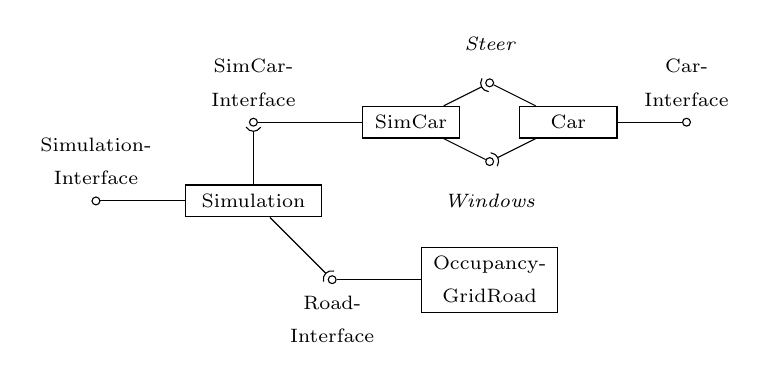
\begin{tikzpicture}[comp/.style   ={rectangle,draw=black, text width=1cm, text centered},
                        if/.style     ={circle   ,draw=black, minimum width=0.1cm, inner sep=0},
                        need/.style   ={-(       ,draw,color=black},
                        provide/.style={-        ,draw, color=black},
                        label/.style  ={rectangle,draw opacity=0, text width=1.5cm, text centered}]

      \coordinate (loff) at(0, 0.5);
      \node[comp, text width=1.5cm]  at(0, 0)              (sim)     {\scriptsize Simulation};
      \node[if]    at($(sim)   -(2, 0)$) (simif)   {};
      \node[label] at($(simif) +(loff)$)           {\scriptsize Simulation\-Interface};
      \node[if]    at($(sim)   +(0, 1)$) (smif)    {};
      \node[label] at($(smif)  +(loff)$)           {\scriptsize SimCar\-Interface};
      \node[if]    at($(sim)   +(1,-1)$) (roadif)  {};
      \node[label] at($(roadif)-(loff)$)           {\scriptsize Road\-Interface};
      \node[comp]  at($(smif)  +(2, 0)$) (simCar)  {\scriptsize SimCar};
      \node[comp, text width=1.5cm]  at($(roadif)+(2, 0)$) (road)    {\scriptsize Occupancy\-GridRoad};
      \node[if]    at($(simCar)+(1, 0.5)$) (cmdif)   {};
      \node[label] at($(cmdif) +(loff)$)           {\it\scriptsize Steer};
      \node[if]    at($(simCar)+(1,-0.5)$) (winif)   {};
      \node[label] at($(winif) -(loff)$)           {\it\scriptsize Windows};
      \node[comp]  at($(simCar)+(2, 0)$) (car)     {\scriptsize Car};
      \node[if]    at($(car)   +(1.5, 0)$) (carif)   {};
      \node[label] at($(carif) +(loff)$)           {\scriptsize Car\-Interface};
      \path[need] (sim)    -- (smif);
      \path[need] (sim)    -- (roadif);
      \path[need] (simCar) -- (cmdif);
      \path[need] (car)    -- (winif);
      \path[provide] (sim)    -- (simif);
      \path[provide] (simCar) -- (smif);
      \path[provide] (road)   -- (roadif);
      \path[provide] (car)    -- (cmdif);
      \path[provide] (simCar) -- (winif);
      \path[provide] (car) -- (carif);
    \end{tikzpicture}
   }
}

\frame{\frametitle{Benefits of Software Components}
  \begin{description}
    \item[Decoupled Devopment]: Developers may focus on a single piece of software. Limits the effects of software changes to the connections between the components. 
    \item[Reusage of Components]: A developed component may be used in any context as long as the interface specifications are fulfilled.
    \item[Easier Testing]: Each component may be tested individually against the specification of its interface, without using any other component
  \end{description}
}

\frame{\frametitle{How to test}
  \begin{block}{The Problem}
    How can the dependancy of a software component be fulfilled without using another component fullfilling the interface.
  \end{block}
  \begin{figure}
    \centering
    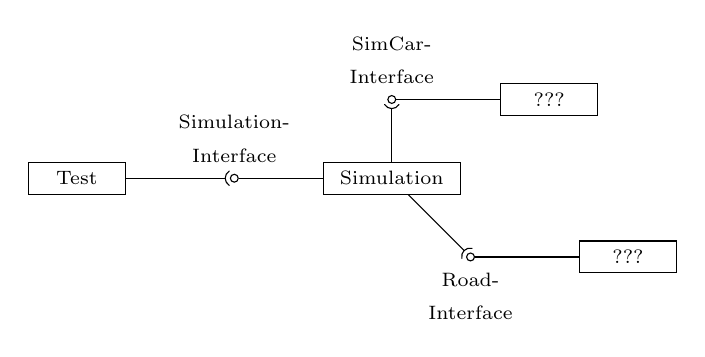
\begin{tikzpicture}[comp/.style   ={rectangle,draw=black, text width=1cm, text centered},
                        if/.style     ={circle   ,draw=black, minimum width=0.1cm, inner sep=0},
                        need/.style   ={-(       ,draw,color=black},
                        provide/.style={-        ,draw, color=black},
                        label/.style  ={rectangle,draw opacity=0, text width=1.5cm, text centered}]

      \coordinate (loff) at(0, 0.5);
      \node[comp, text width=1.5cm]  at(0, 0)              (sim)     {\scriptsize Simulation};
      \node[if]    at($(sim)   -(2, 0)$) (simif)   {};
      \node[label] at($(simif) +(loff)$)           {\scriptsize Simulation\-Interface};
      \node[comp]  at($(sim)   -(4, 0)$) (test)    {\scriptsize Test};
      \node[if]    at($(sim)   +(0, 1)$) (smif)    {};
      \node[label] at($(smif)  +(loff)$)           {\scriptsize SimCar\-Interface};
      \node[if]    at($(sim)   +(1,-1)$) (roadif)  {};
      \node[label] at($(roadif)-(loff)$)           {\scriptsize Road\-Interface};
      \node[comp]  at($(smif)  +(2, 0)$) (simCar)  {\scriptsize ???};
      \node[comp]  at($(roadif)+(2, 0)$) (road)    {\scriptsize ???};
      \path[need] (sim)    -- (smif);
      \path[need] (test)   -- (simif);
      \path[need] (sim)    -- (roadif);
      \path[provide] (sim)    -- (simif);
      \path[provide] (simCar) -- (smif);
      \path[provide] (road)   -- (roadif);
    \end{tikzpicture}
    \caption{ROS Example Simulation Testing Challenge}
  \end{figure}
}

\section{GMock}

\frame{\frametitle{Solutions}
  \begin{block}{Definition: Fake Object}
    Fake objects have working implementations, but usually take some shortcut (perhaps to make the operations less expensive), which makes them not suitable for production. An in-memory file system would be an example of a fake.\footnotemark[1]  \end{block}
  \pause
  \begin{block}{Definition: Mock Object}
    Mocks are objects pre-programmed with expectations, which form a specification of the calls they are expected to receive.\footnotemark[1]
  \end{block}
  \footnotetext[1]{GMock for Dummies: \url{https://code.google.com/p/googlemock/wiki/ForDummies}}
}

\begin{frame}[fragile]
\frametitle{Mocking an Object}
  \begin{block}{Mock Methods}
    A Mock Method replaces the abstract or incomplete implementation of a {\bf virtual} method of a base class. It is defined without any implementation while fulfilling the class' interface.
  \end{block}
  \begin{lstlisting}[title=RoadInterface Mock Class, style=code, basicstyle=\ttfamily\footnotesize\color{white}]
class MockRoad : public RoadInterface {
  public:
    MockRoad(unsigned int maxY, unsigned int maxX)
      : RoadInterface(maxY, maxX) {}
    MOCK_METHOD3(writeCell, void(unsigned int y, 
                                 unsigned int x, Cell cell));
    MOCK_CONST_METHOD2(readCell, Cell(unsigned int y,
                                      unsigned int x));
    MOCK_CONST_METHOD2(isFree, bool(unsigned int y, 
                                    unsigned int x));
};
  \end{lstlisting}
\end{frame}

\begin{frame}[fragile]
  \frametitle{Expectations in Value}
  \begin{description}
    \item[\tt EXPECT\_CALL] declares a Mock Method to be expected to be called
    \item[\tt Lt] is a {\it Matcher} comparing provided arguments to be {\bf L}ower {\bf t}hen a reference.
    \item[\tt \_] is the wildcard {\it Matcher} stating all arguments should be matched.
   \end{description}
  \begin{lstlisting}[title=Expecations on Value Example, style=code, basicstyle=\ttfamily\footnotesize\color{white}]
  using ::testing::Lt;
  using ::testing::_;

  EXPECT_CALL(road, isFree(Lt(road.maxY()),
                           Lt(road.maxX())
                           ));
  EXPECT_CALL(road, writeCell(_, _, 
                              RoadInterface::Cell::Car
                              ));
  \end{lstlisting}
\end{frame}

\begin{frame}[fragile]
  \frametitle{Expectations in Time}
  \begin{description}
    \item[\tt .Times()] declares the expected number of calls to a mock method with the specified arguments
    \item[\tt AtLeast()] declares a minimum amount
  \end{description}
  \begin{lstlisting}[title=Expectations on Time Example, style=code, basicstyle=\ttfamily\footnotesize\color{white}]
using ::testing::AtLeast;

Test(SimulationTest, carCreationTest) {
  MockRoad road(10, 10);
  
  EXPECT_CALL(road, isFree(_, _))
    .Times(AtLeast(1))
  EXPECT_CALL(road, writeCell(_, _, _))
    .Times(1);

  Simulation<MockCar> sim(road);
  sim.createCar("TestCar");
}
  \end{lstlisting}

\end{frame}

\begin{frame}[fragile]
  \frametitle{Returning Values}
  \begin{description}
    \item[\tt .WillOnce()]: Modifies the Mock Method to do an {\bf Action} a single time
    \item[\tt .WillRepeatedly()]: Modifies the Mock Method to do an {\bf Action} all the time
    \item[\tt Return()]: return the specifies value as the {\bf Action}
  \end{description}

  \begin{lstlisting}[title=Example of a Return Action, style=code, basicstyle=\ttfamily\footnotesize\color{white}]
  using ::testing::Return;
  MockRoad mRoad(10, 10);
  EXPECT_CALL(road, isFree(Lt(road.maxY()),
                           Lt(road.maxX())))
    .Times(AtLeast(1))
    .WillOnce(Return(true))
    .WillRepeatedly(Return(false));
  \end{lstlisting}
\end{frame}


\begin{frame}[fragile]
  \frametitle{Side Effects}
  \begin{description}
    \item[Assign(T* ptr, T v)]: assigns {\tt v} to the address {\tt ptr} as  the methods action
  \end{description}
  \begin{lstlisting}[title=Example of a Side-Effect Action, style=code, basicstyle=\ttfamily\footnotesize\color{white}]
class MockCar : public SimCarInterface {
  public:
    MOCK_METHOD1(x, void(unsigned int x));

    MockCar(const string& numberPlate, Dir dir, 
            unsigned int y, unsigned int x)
      : SimCarInterface(numberPlate, dir, 1, 1) {
      EXPECT_CALL(*this, x(2))
        .Times(AtLeast(1))
        .WillRepeatedly(Assign(&mX, 2));
      }
};
  \end{lstlisting}
  \footnotetext{Many more actions and receipes can be found in the cookbook: \url{https://code.google.com/p/googlemock/wiki/CookBook}}
\end{frame}


\begin{frame}[fragile]
  \frametitle{Catkin Integration}
  \begin{block}{No Default Catkin Integration}
    Unfortunately; there is currently no GMock integration within catkin available. Therefore, a workaround needs to be used.
  \end{block}

  \begin{lstlisting}[title=GMock Catkin Integration Workaround, style=code, language=python, basicstyle=\ttfamily\footnotesize\color{white}]
if(CATKIN_ENABLE_TESTING)

  # Create a gmock target to be used as a dependency
  # by test programs
  add_library(gmock IMPORTED STATIC GLOBAL)
  set_property(TARGET gmock PROPERTY IMPORTED_LOCATION
              /usr/lib/libgmock.so)

  # Add gtest based cpp test target and link libraries
  catkin_add_gtest(${PROJECT_NAME}-mock src/Mock.cpp)
  target_link_libraries(${PROJECT_NAME}-mock 
                        ${catkin_LIBRARIES} cars gmock)

endif()
  \end{lstlisting}
\end{frame}

\section{Finding Regressions}
\frame{\frametitle{VCS History}

}

\frame{\frametitle{Rewriting History}

}

\frame{\frametitle{Reverting and Blaming}

}

\section{Still ToDo}

\frame{\frametitle{Left Overs}

\begin{itemize}
  \item Runtime Testing using Ros::SelfTest
\end{itemize}

}
\end{document}
